%%%%%%%%%%%%%%%%%%%%%%%%%%%%%%%%%%%%%%%%%
% The Legrand Orange Book (Black Edition)
% LaTeX Template
% Version 2.0 (9/2/15)
%
% This template has been downloaded from:
% http://www.LaTeXTemplates.m
%
% Mathias Legrand (legrand.mathias@gmail.com) with modifications by:
% Vel (vel@latextemplates.com)
% Jose Carlos Garcia (jose.carlos.garcia.95@gmail.com) (Black Edition)
% License:
% CC BY-NC-SA 3.0 (http://creativecommons.org/licenses/by-nc-sa/3.0/)
%
% Compiling this template:
% This template uses biber for its bibliography and makeindex for its index.
% When you first open the template, compile it from the command line with the 
% commands below to make sure your LaTeX distribution is configured correctly:
%
% 1) pdflatex main
% 2) makeindex main.idx -s StyleInd.ist
% 3) biber main
% 4) pdflatex main x 2
%
% After this, when you wish to update the bibliography/index use the appropriate
% command above and make sure to compile with pdflatex several times 
% afterwards to propagate your changes to the document.
%
% This template also uses a number of packages which may need to be
% updated to the newest versions for the template to compile. It is strongly
% recommended you update your LaTeX distribution if you have any
% compilation errors.
%
% Important note:
% Chapter heading images should have a 2:1 width:height ratio,
% e.g. 920px width and 460px height.
%
%%%%%%%%%%%%%%%%%%%%%%%%%%%%%%%%%%%%%%%%%

%----------------------------------------------------------------------------------------
%	PACKAGES AND OTHER DOCUMENT CONFIGURATIONS
%----------------------------------------------------------------------------------------

\documentclass[11pt,fleqn]{book} % Default font size and left-justified equations
% Acentos %
\usepackage[spanish]{babel}
\selectlanguage{spanish}
\usepackage[utf8]{inputenc}

% Matematicas %
\usepackage{amsmath}
\usepackage{amsfonts}
\usepackage{amsthm}


%Enlaces%

%----------------------------------------------------------------------------------------

%%%%%%%%%%%%%%%%%%%%%%%%%%%%%%%%%%%%%%%%%
% The Legrand Orange Book
% Structural Definitions File
% Version 2.0 (9/2/15)
%
% Original author:
% Mathias Legrand (legrand.mathias@gmail.com) with modifications by:
% Vel (vel@latextemplates.com)
% 
% This file has been downloaded from:
% http://www.LaTeXTemplates.com
%
% License:
% CC BY-NC-SA 3.0 (http://creativecommons.org/licenses/by-nc-sa/3.0/)
%
%%%%%%%%%%%%%%%%%%%%%%%%%%%%%%%%%%%%%%%%%

%----------------------------------------------------------------------------------------
%	VARIOUS REQUIRED PACKAGES AND CONFIGURATIONS
%----------------------------------------------------------------------------------------

\usepackage[top=3cm,bottom=3cm,left=3cm,right=3cm,headsep=10pt,a4paper]{geometry} % Page margins

\usepackage{graphicx} % Required for including pictures
\graphicspath{{Pictures/}} % Specifies the directory where pictures are stored

\usepackage{lipsum} % Inserts dummy text
\usepackage{wrapfig}
\usepackage{caption}
\usepackage{subcaption}
\usepackage{tikz} % Required for drawing custom shapes

\usepackage[spanish]{babel} % English language/hyphenation

\usepackage{enumitem} % Customize lists
\setlist{nolistsep} % Reduce spacing between bullet points and numbered lists

\usepackage{booktabs} % Required for nicer horizontal rules in tables

\usepackage{xcolor} % Required for specifying colors by name
\definecolor{ocre}{RGB}{243,102,25} % Define the orange color used for highlighting throughout the book
\definecolor{darkjose}{HTML}{4a4a4a}
\usepackage{array,bm}

\newcolumntype{R}{>{$}r<{$}}
\newcolumntype{C}{>{$}c<{$}}
\renewcommand{\arraystretch}{1.2}
%----------------------------------------------------------------------------------------
%	FONTS
%----------------------------------------------------------------------------------------

\usepackage{avant} % Use the Avantgarde font for headings
%\usepackage{times} % Use the Times font for headings
\usepackage{mathptmx} % Use the Adobe Times Roman as the default text font together with math symbols from the Sym­bol, Chancery and Com­puter Modern fonts

\usepackage{microtype} % Slightly tweak font spacing for aesthetics
\usepackage[utf8]{inputenc} % Required for including letters with accents
\usepackage[T1]{fontenc} % Use 8-bit encoding that has 256 glyphs

%----------------------------------------------------------------------------------------
%	BIBLIOGRAPHY AND INDEX
%----------------------------------------------------------------------------------------

\usepackage[style=alphabetic,citestyle=numeric,sorting=nyt,sortcites=true,autopunct=true,babel=hyphen,hyperref=true,abbreviate=false,backref=true,backend=biber]{biblatex}
\addbibresource{bibliography.bib} % BibTeX bibliography file
\defbibheading{bibempty}{}

\usepackage{calc} % For simpler calculation - used for spacing the index letter headings correctly
\usepackage{makeidx} % Required to make an index
\makeindex % Tells LaTeX to create the files required for indexing

%----------------------------------------------------------------------------------------
%	MAIN TABLE OF CONTENTS
%----------------------------------------------------------------------------------------

\usepackage{titletoc} % Required for manipulating the table of contents

\contentsmargin{0cm} % Removes the default margin

% Part text styling
\titlecontents{part}[0cm]
{\addvspace{20pt}\centering\large\bfseries}
{}
{}
{}

% Chapter text styling
\titlecontents{chapter}[1.25cm] % Indentation
{\addvspace{12pt}\large\sffamily\bfseries} % Spacing and font options for chapters
{\color{darkjose!60}\contentslabel[\Large\thecontentslabel]{1.25cm}\color{darkjose}} % Chapter number
{\color{darkjose}}  
{\color{darkjose!60}\normalsize\;\titlerule*[.5pc]{.}\;\thecontentspage} % Page number

% Section text styling
\titlecontents{section}[1.25cm] % Indentation
{\addvspace{3pt}\sffamily\bfseries} % Spacing and font options for sections
{\contentslabel[\thecontentslabel]{1.25cm}} % Section number
{}
{\hfill\color{black}\thecontentspage} % Page number
[]

% Subsection text styling
\titlecontents{subsection}[1.25cm] % Indentation
{\addvspace{1pt}\sffamily\small} % Spacing and font options for subsections
{\contentslabel[\thecontentslabel]{1.25cm}} % Subsection number
{}
{\ \titlerule*[.5pc]{.}\;\thecontentspage} % Page number
[]

% List of figures
\titlecontents{figure}[0em]
{\addvspace{-5pt}\sffamily}
{\thecontentslabel\hspace*{1em}}
{}
{\ \titlerule*[.5pc]{.}\;\thecontentspage}
[]

% List of tables
\titlecontents{table}[0em]
{\addvspace{-5pt}\sffamily}
{\thecontentslabel\hspace*{1em}}
{}
{\ \titlerule*[.5pc]{.}\;\thecontentspage}
[]

%----------------------------------------------------------------------------------------
%	MINI TABLE OF CONTENTS IN PART HEADS
%----------------------------------------------------------------------------------------

% Chapter text styling
\titlecontents{lchapter}[0em] % Indenting
{\addvspace{15pt}\large\sffamily\bfseries} % Spacing and font options for chapters
{\color{darkjose}\contentslabel[\Large\thecontentslabel]{1.25cm}\color{darkjose}} % Chapter number
{}  
{\color{darkjose}\normalsize\sffamily\bfseries\;\titlerule*[.5pc]{.}\;\thecontentspage} % Page number

% Section text styling
\titlecontents{lsection}[0em] % Indenting
{\sffamily\small} % Spacing and font options for sections
{\contentslabel[\thecontentslabel]{1.25cm}} % Section number
{}
{}

% Subsection text styling
\titlecontents{lsubsection}[.5em] % Indentation
{\normalfont\footnotesize\sffamily} % Font settings
{}
{}
{}

%----------------------------------------------------------------------------------------
%	PAGE HEADERS
%----------------------------------------------------------------------------------------

\usepackage{fancyhdr} % Required for header and footer configuration

\pagestyle{fancy}
\renewcommand{\chaptermark}[1]{\markboth{\sffamily\normalsize\bfseries\chaptername\ \thechapter.\ #1}{}} % Chapter text font settings
\renewcommand{\sectionmark}[1]{\markright{\sffamily\normalsize\thesection\hspace{5pt}#1}{}} % Section text font settings
\fancyhf{} \fancyhead[LE,RO]{\sffamily\normalsize\thepage} % Font setting for the page number in the header
\fancyhead[LO]{\rightmark} % Print the nearest section name on the left side of odd pages
\fancyhead[RE]{\leftmark} % Print the current chapter name on the right side of even pages
\renewcommand{\headrulewidth}{0.5pt} % Width of the rule under the header
\addtolength{\headheight}{2.5pt} % Increase the spacing around the header slightly
\renewcommand{\footrulewidth}{0pt} % Removes the rule in the footer
\fancypagestyle{plain}{\fancyhead{}\renewcommand{\headrulewidth}{0pt}} % Style for when a plain pagestyle is specified

% Removes the header from odd empty pages at the end of chapters
\makeatletter
\renewcommand{\cleardoublepage}{
	\clearpage\ifodd\c@page\else
	\hbox{}
	\vspace*{\fill}
	\thispagestyle{empty}
	\newpage
	\fi}

%----------------------------------------------------------------------------------------
%	THEOREM STYLES
%----------------------------------------------------------------------------------------

\usepackage{amsmath,amsfonts,amssymb,amsthm} % For math equations, theorems, symbols, etc

\newcommand{\intoo}[2]{\mathopen{]}#1\,;#2\mathclose{[}}
\newcommand{\ud}{\mathop{\mathrm{{}d}}\mathopen{}}
\newcommand{\intff}[2]{\mathopen{[}#1\,;#2\mathclose{]}}
\newtheorem{notation}{Notation}[chapter]

% Boxed/framed environments
\newtheoremstyle{darkjosenumbox}% % Theorem style name
{0pt}% Space above
{0pt}% Space below
{\normalfont}% % Body font
{}% Indent amount
{\small\bf\sffamily\color{darkjose}}% % Theorem head font
{\;}% Punctuation after theorem head
{0.25em}% Space after theorem head
{\small\sffamily\color{darkjose}\thmname{#1}\nobreakspace\thmnumber{\@ifnotempty{#1}{}\@upn{#2}}% Theorem text (e.g. Theorem 2.1)
	\thmnote{\nobreakspace\the\thm@notefont\sffamily\bfseries\color{black}---\nobreakspace#3.}} % Optional theorem note
\renewcommand{\qedsymbol}{$\blacksquare$}% Optional qed square

\newtheoremstyle{blacknumex}% Theorem style name
{5pt}% Space above
{5pt}% Space below
{\normalfont}% Body font
{} % Indent amount
{\small\bf\sffamily}% Theorem head font
{\;}% Punctuation after theorem head
{0.25em}% Space after theorem head
{\small\sffamily{\tiny\ensuremath{\blacksquare}}\nobreakspace\thmname{#1}\nobreakspace\thmnumber{\@ifnotempty{#1}{}\@upn{#2}}% Theorem text (e.g. Theorem 2.1)
	\thmnote{\nobreakspace\the\thm@notefont\sffamily\bfseries---\nobreakspace#3.}}% Optional theorem note

\newtheoremstyle{blacknumbox} % Theorem style name
{0pt}% Space above
{0pt}% Space below
{\normalfont}% Body font
{}% Indent amount
{\small\bf\sffamily}% Theorem head font
{\;}% Punctuation after theorem head
{0.25em}% Space after theorem head
{\small\sffamily\thmname{#1}\nobreakspace\thmnumber{\@ifnotempty{#1}{}\@upn{#2}}% Theorem text (e.g. Theorem 2.1)
	\thmnote{\nobreakspace\the\thm@notefont\sffamily\bfseries---\nobreakspace#3.}}% Optional theorem note

% Non-boxed/non-framed environments
\newtheoremstyle{darkjosenum}% % Theorem style name
{5pt}% Space above
{5pt}% Space below
{\normalfont}% % Body font
{}% Indent amount
{\small\bf\sffamily\color{darkjose}}% % Theorem head font
{\;}% Punctuation after theorem head
{0.25em}% Space after theorem head
{\small\sffamily\color{darkjose}\thmname{#1}\nobreakspace\thmnumber{\@ifnotempty{#1}{}\@upn{#2}}% Theorem text (e.g. Theorem 2.1)
	\thmnote{\nobreakspace\the\thm@notefont\sffamily\bfseries\color{black}---\nobreakspace#3.}} % Optional theorem note
\renewcommand{\qedsymbol}{$\blacksquare$}% Optional qed square
\makeatother

% Defines the theorem text style for each type of theorem to one of the three styles above
\newcounter{dummy} 
\numberwithin{dummy}{section}
\theoremstyle{darkjosenumbox}
\newtheorem{theoremeT}[dummy]{Teorema}
\newtheorem{problem}{Problem}[chapter]
\newtheorem{exerciseT}{Exercise}[chapter]
\theoremstyle{blacknumex}
\newtheorem{exampleT}{Example}[chapter]
\theoremstyle{blacknumbox}
\newtheorem{vocabulary}{Vocabulary}[chapter]
\newtheorem{definitionT}{Definición}[section]
\newtheorem{corollaryT}[dummy]{Corolario}
\theoremstyle{darkjosenum}
\newtheorem{proposition}[dummy]{Proposición}

%----------------------------------------------------------------------------------------
%	DEFINITION OF COLORED BOXES
%----------------------------------------------------------------------------------------

\RequirePackage[framemethod=default]{mdframed} % Required for creating the theorem, definition, exercise and corollary boxes

% Theorem box
\newmdenv[skipabove=7pt,
skipbelow=7pt,
backgroundcolor=black!5,
linecolor=darkjose,
innerleftmargin=5pt,
innerrightmargin=5pt,
innertopmargin=5pt,
leftmargin=0cm,
rightmargin=0cm,
innerbottommargin=5pt]{tBox}

% Exercise box	  
\newmdenv[skipabove=7pt,
skipbelow=7pt,
rightline=false,
leftline=true,
topline=false,
bottomline=false,
backgroundcolor=darkjose!10,
linecolor=darkjose,
innerleftmargin=5pt,
innerrightmargin=5pt,
innertopmargin=5pt,
innerbottommargin=5pt,
leftmargin=0cm,
rightmargin=0cm,
linewidth=4pt]{eBox}	

% Definition box
\newmdenv[skipabove=7pt,
skipbelow=7pt,
rightline=false,
leftline=true,
topline=false,
bottomline=false,
linecolor=darkjose,
innerleftmargin=5pt,
innerrightmargin=5pt,
innertopmargin=0pt,
leftmargin=0cm,
rightmargin=0cm,
linewidth=4pt,
innerbottommargin=0pt]{dBox}	

% Corollary box
\newmdenv[skipabove=7pt,
skipbelow=7pt,
rightline=false,
leftline=true,
topline=false,
bottomline=false,
linecolor=gray,
backgroundcolor=black!5,
innerleftmargin=5pt,
innerrightmargin=5pt,
innertopmargin=5pt,
leftmargin=0cm,
rightmargin=0cm,
linewidth=4pt,
innerbottommargin=5pt]{cBox}

% Creates an environment for each type of theorem and assigns it a theorem text style from the "Theorem Styles" section above and a colored box from above
\newenvironment{theorem}{\begin{tBox}\begin{theoremeT}}{\end{theoremeT}\end{tBox}}
\newenvironment{exercise}{\begin{eBox}\begin{exerciseT}}{\hfill{\color{darkjose}\tiny\ensuremath{\blacksquare}}\end{exerciseT}\end{eBox}}				  
\newenvironment{definition}{\begin{dBox}\begin{definitionT}}{\end{definitionT}\end{dBox}}	
\newenvironment{example}{\begin{exampleT}}{\hfill{\tiny\ensuremath{\blacksquare}}\end{exampleT}}		
\newenvironment{corollary}{\begin{cBox}\begin{corollaryT}}{\end{corollaryT}\end{cBox}}	

%----------------------------------------------------------------------------------------
%	REMARK ENVIRONMENT
%----------------------------------------------------------------------------------------

\newenvironment{remark}{\par\vspace{10pt}\small % Vertical white space above the remark and smaller font size
	\begin{list}{}{
			\leftmargin=35pt % Indentation on the left
			\rightmargin=25pt}\item\ignorespaces % Indentation on the right
		\makebox[-2.5pt]{\begin{tikzpicture}[overlay]
			\node[draw=darkjose!60,line width=1pt,circle,fill=darkjose!25,font=\sffamily\bfseries,inner sep=2pt,outer sep=0pt] at (-15pt,0pt){\textcolor{darkjose}{R}};\end{tikzpicture}} % Orange R in a circle
		\advance\baselineskip -1pt}{\end{list}\vskip5pt} % Tighter line spacing and white space after remark

%----------------------------------------------------------------------------------------
%	SECTION NUMBERING IN THE MARGIN
%----------------------------------------------------------------------------------------

\makeatletter
\renewcommand{\@seccntformat}[1]{\llap{\textcolor{darkjose}{\csname the#1\endcsname}\hspace{1em}}}                    
\renewcommand{\section}{\@startsection{section}{1}{\z@}
	{-4ex \@plus -1ex \@minus -.4ex}
	{1ex \@plus.2ex }
	{\normalfont\large\sffamily\bfseries}}
\renewcommand{\subsection}{\@startsection {subsection}{2}{\z@}
	{-3ex \@plus -0.1ex \@minus -.4ex}
	{0.5ex \@plus.2ex }
	{\normalfont\sffamily\bfseries}}
\renewcommand{\subsubsection}{\@startsection {subsubsection}{3}{\z@}
	{-2ex \@plus -0.1ex \@minus -.2ex}
	{.2ex \@plus.2ex }
	{\normalfont\small\sffamily\bfseries}}                        
\renewcommand\paragraph{\@startsection{paragraph}{4}{\z@}
	{-2ex \@plus-.2ex \@minus .2ex}
	{.1ex}
	{\normalfont\small\sffamily\bfseries}}

%----------------------------------------------------------------------------------------
%	PART HEADINGS
%----------------------------------------------------------------------------------------

% numbered part in the table of contents
\newcommand{\@mypartnumtocformat}[2]{%
	\setlength\fboxsep{0pt}%
	\noindent\colorbox{darkjose!20}{\strut\parbox[c][.7cm]{\ecart}{\color{darkjose!70}\Large\sffamily\bfseries\centering#1}}\hskip\esp\colorbox{darkjose!40}{\strut\parbox[c][.7cm]{\linewidth-\ecart-\esp}{\Large\sffamily\centering#2}}}%
%%%%%%%%%%%%%%%%%%%%%%%%%%%%%%%%%%
% unnumbered part in the table of contents
\newcommand{\@myparttocformat}[1]{%
	\setlength\fboxsep{0pt}%
	\noindent\colorbox{darkjose!40}{\strut\parbox[c][.7cm]{\linewidth}{\Large\sffamily\centering#1}}}%
%%%%%%%%%%%%%%%%%%%%%%%%%%%%%%%%%%
\newlength\esp
\setlength\esp{4pt}
\newlength\ecart
\setlength\ecart{1.2cm-\esp}
\newcommand{\thepartimage}{}%
\newcommand{\partimage}[1]{\renewcommand{\thepartimage}{#1}}%
\def\@part[#1]#2{%
	\ifnum \c@secnumdepth >-2\relax%
	\refstepcounter{part}%
	\addcontentsline{toc}{part}{\texorpdfstring{\protect\@mypartnumtocformat{\thepart}{#1}}{\partname~\thepart\ ---\ #1}}
	\else%
	\addcontentsline{toc}{part}{\texorpdfstring{\protect\@myparttocformat{#1}}{#1}}%
	\fi%
	\startcontents%
	\markboth{}{}%
	{\thispagestyle{empty}%
		\begin{tikzpicture}[remember picture,overlay]%
		\node at (current page.north west){\begin{tikzpicture}[remember picture,overlay]%	
			\fill[darkjose!20](0cm,0cm) rectangle (\paperwidth,-\paperheight);
			\node[anchor=north] at (4cm,-3.25cm){\color{darkjose!40}\fontsize{220}{100}\sffamily\bfseries\@Roman\c@part}; 
			\node[anchor=south east] at (\paperwidth-1cm,-\paperheight+1cm){\parbox[t][][t]{8.5cm}{
					\printcontents{l}{0}{\setcounter{tocdepth}{1}}%
			}};
			\node[anchor=north east] at (\paperwidth-1.5cm,-3.25cm){\parbox[t][][t]{15cm}{\strut\raggedleft\color{white}\fontsize{30}{30}\sffamily\bfseries#2}};
			\end{tikzpicture}};
\end{tikzpicture}}%
\@endpart}
\def\@spart#1{%
\startcontents%
\phantomsection
{\thispagestyle{empty}%
	\begin{tikzpicture}[remember picture,overlay]%
	\node at (current page.north west){\begin{tikzpicture}[remember picture,overlay]%	
		\fill[darkjose!20](0cm,0cm) rectangle (\paperwidth,-\paperheight);
		\node[anchor=north east] at (\paperwidth-1.5cm,-3.25cm){\parbox[t][][t]{15cm}{\strut\raggedleft\color{white}\fontsize{30}{30}\sffamily\bfseries#1}};
		\end{tikzpicture}};
\end{tikzpicture}}
\addcontentsline{toc}{part}{\texorpdfstring{%
	\setlength\fboxsep{0pt}%
	\noindent\protect\colorbox{darkjose!40}{\strut\protect\parbox[c][.7cm]{\linewidth}{\Large\sffamily\protect\centering #1\quad\mbox{}}}}{#1}}%
\@endpart}
\def\@endpart{\vfil\newpage
\if@twoside
\if@openright
\null
\thispagestyle{empty}%
\newpage
\fi
\fi
\if@tempswa
\twocolumn
\fi}

%----------------------------------------------------------------------------------------
%	CHAPTER HEADINGS
%----------------------------------------------------------------------------------------

\newcommand{\thechapterimage}{}%
\newcommand{\chapterimage}[1]{\renewcommand{\thechapterimage}{#1}}%
\def\@makechapterhead#1{%
{\parindent \z@ \raggedright \normalfont 
\ifnum \c@secnumdepth >\m@ne
\if@mainmatter
\begin{tikzpicture}[remember picture,overlay]
\node at (current page.north west)
{\begin{tikzpicture}[remember picture,overlay]
	\node[anchor=north west,inner sep=0pt] at (0,0) {\includegraphics[width=\paperwidth]{\thechapterimage}};
	\draw[anchor=west] (\Gm@lmargin,-9cm) node [line width=2pt,rounded corners=7pt,draw=darkjose,fill=white,fill opacity=0.5,inner sep=15pt]{\strut\makebox[22cm]{}};
	\draw[anchor=west] (\Gm@lmargin+.3cm,-9cm) node {\huge\sffamily\bfseries\color{black}\thechapter. #1\strut};
	\end{tikzpicture}};
\end{tikzpicture}
\else
\begin{tikzpicture}[remember picture,overlay]
\node at (current page.north west)
{\begin{tikzpicture}[remember picture,overlay]
\node[anchor=north west,inner sep=0pt] at (0,0) {\includegraphics[width=\paperwidth]{\thechapterimage}};
\draw[anchor=west] (\Gm@lmargin,-9cm) node [line width=2pt,rounded corners=7pt,draw=darkjose,fill=white,fill opacity=0.5,inner sep=15pt]{\strut\makebox[22cm]{}};
\draw[anchor=west] (\Gm@lmargin+.3cm,-9cm) node {\huge\sffamily\bfseries\color{black}#1\strut};
\end{tikzpicture}};
\end{tikzpicture}
\fi\fi\par\vspace*{270\p@}}}

%-------------------------------------------

\def\@makeschapterhead#1{%
\begin{tikzpicture}[remember picture,overlay]
\node at (current page.north west)
{\begin{tikzpicture}[remember picture,overlay]
\node[anchor=north west,inner sep=0pt] at (0,0) {\includegraphics[width=\paperwidth]{\thechapterimage}};
\draw[anchor=west] (\Gm@lmargin,-9cm) node [line width=2pt,rounded corners=7pt,draw=darkjose,fill=white,fill opacity=0.5,inner sep=15pt]{\strut\makebox[22cm]{}};
\draw[anchor=west] (\Gm@lmargin+.3cm,-9cm) node {\huge\sffamily\bfseries\color{black}#1\strut};
\end{tikzpicture}};
\end{tikzpicture}
\par\vspace*{270\p@}}
\makeatother

%----------------------------------------------------------------------------------------
%	HYPERLINKS IN THE DOCUMENTS
%----------------------------------------------------------------------------------------

\usepackage{hyperref}
\hypersetup{hidelinks,backref=true,pagebackref=true,hyperindex=true,colorlinks=false,breaklinks=true,urlcolor= darkjose,bookmarks=true,bookmarksopen=false,pdftitle={Title},pdfauthor={Author}}
\usepackage{bookmark}
\bookmarksetup{
open,
numbered,
addtohook={%
\ifnum\bookmarkget{level}=0 % chapter
\bookmarksetup{bold}%
\fi
\ifnum\bookmarkget{level}=-1 % part
\bookmarksetup{color=darkjose,bold}%
\fi
}
}

%
% Keyboard
%
\usepackage{menukeys} % Insert the commands.tex file which contains the majority of the structure behind the template

\begin{document}

%----------------------------------------------------------------------------------------
%	TITLE PAGE
%----------------------------------------------------------------------------------------

\begingroup
\thispagestyle{empty}
\begin{tikzpicture}[remember picture,overlay]
\coordinate [below=12cm] (midpoint) at (current page.north);
\node at (current page.north west)
{\begin{tikzpicture}[remember picture,overlay]
	\node[anchor=north west,inner sep=0pt] at (0,0) {
\includegraphics[height=\paperheight]{Wallpaper}}; % Background image
	\draw[anchor=north] (midpoint) node [fill=darkjose!30!white,fill opacity=0.6,text opacity=1,inner sep=1cm]{\Huge\centering\bfseries\sffamily\parbox[c][][t]{\paperwidth}{\centering Apuntes Progamación Matemática\\[15pt] % Book title
			{\huge Escrito por Jose Carlos García}}}; % Author name
	\end{tikzpicture}};
\end{tikzpicture}
\vfill
\endgroup
\newpage
\textit{Los presentes apuntes han sido escrito por José Carlos García Ortega bajo la licencia GNU General Public License. Cualquier persona puede modificar, descargar y compartir cualquier modificación de este documento.\\ \\
Por otro lado, los profesores de la asignatura no tienen \textbf{ninguna responsabilidad acerca de la revisión de estos apuntes}.\\ \\
Estos apuntes han sido escrito basados en las clases de Programación Matemática del curso 2016-2017 del Grado de Matemáticas en la Universidad de Cádiz.}

%----------------------------------------------------------------------------------------
%	TABLE OF CONTENTS
%----------------------------------------------------------------------------------------


\chapterimage{indice} % Table of contents heading image

\pagestyle{empty} % No headers

\tableofcontents % Print the table of contents itself

% \cleardoublepage % Forces the first chapter to start on an odd page so it's on the right


\setlength{\parindent}{0pt} % Default is 15pt.


\pagestyle{fancy} % Print headers again

%----------------------------------------------------------------------------------------
%	PART
%----------------------------------------------------------------------------------------

\part{Tema 1:}

%----------------------------------------------------------------------------------------
%	CHAPTER 1
%----------------------------------------------------------------------------------------

\chapterimage{capitulo1} % Chapter heading image

\chapter{Búsqueda de máximos y mínimos.}
\section{Funciones lineales}\index{Funciones lineales}
En primer lugar definimos el concepto de función lineal, que nos ayudará a definir el concepto \textit{problema de programación lineal}
\begin{definition}[Función lineal]
	Dada una función $f: D\subset\mathbb{R}^n \longrightarrow \mathbb{R}$ se dice que es lineal si cumple lo siguiente:
	\begin{align}
		f(\alpha x + \beta y) = \alpha f(x) + \beta f(y)
	\end{align}
	Donde $x, y \in D$ son variables y $\alpha, \beta \in \mathbb{R}$ son constantes reales.
\end{definition}
En general, una función lineal $f: D\subset \mathbb{R}^n \longrightarrow \mathbb{R}$ vendrá definida de la siguiente forma:
\begin{align}
f(x_1,x_2,...,x_n)=c_1x_1+c_2+x_2+...+c_nx_n
\end{align}
\newpage
\section{Problema de programación lineal}
Una vez definido lo que es una función lineal, definimos el concepto de \textit{problema de programación lineal}.

\begin{definition}[Problema de programación lineal]
	Un problema de programación lineal (PPL) es un problema matemático que se puede expresar de la siguiente forma: \\
	Hallar el máximo / mínimo de una función lineal, $f(x)=c_1x_1+c_2+x_2+...+c_nx_n$ sujeto a una serie de restricciones que podemos expresar como:
	\begin{equation*}
	\left\lbrace
	\begin{array}{l}
	a_{11}x_1+a_{12}x_2+...+a_{1n}x_n \leq b_1 \\
	... \\
	a_{s1}x_1+a_{s2}x_2+...+a_{sn}x_n \leq b_s \\
	... \\
	a_{t1}x_1+a_{t2}x_2+...+a_{tn}x_n \leq b_t \\
	... \\
	a_{t+1,1}x_1+a_{t+1,2}x_2+...+a_{t+1,n}x_n = b_{t+1} \\
	... \\
	a_{m1}x_1+a_{m2}x_2+...+a_{mn}x_n = b_{m}
	\end{array}
	\right.
	\end{equation*}
	Donde $x_i, a_{ij}, b_j \in \mathbb{R}$ para todo $1\leq i \leq n$, $1 \leq j \leq m$. \\
	Nótese que lo que expresa entre llaves corresponde a una restricción que puede ser hecha a través de desigualdades o igualdades.
\end{definition}
Por otro lado, para evitar problemas con las desigualdades, todas estas restricciones se pueden escribir como igualdades que cumplen ciertas propiedades. \\
Cuando sucede esto, decimos que nuestro problema de programación lineal está expresado en formato estándar.

\begin{definition}[Problema de programación lineal estándar]
	Un PPL está expresado en formato estándar si se puede escribir como: \\
		Hallar el máximo / mínimo de una función lineal, $f(x)=c_1x_1+c_2+x_2+...+c_nx_n$ sujeto a una serie de restricciones que podemos expresar como:
		\begin{equation*}
		\left\lbrace
		\begin{array}{l}
		a_{11}x_1+a_{12}x_2+...+a_{1n}x_n = b_1 \\
		a_{21}x_1+a_{22}x_2+...+a_{2n}x_n = b_2 \\
		... \\
		a_{m1}x_1+a_{m2}x_2+...+a_{mn}x_n = b_{m}
		\end{array}
		\right.
		\end{equation*}
		Donde $x_i, b_j \in \mathbb{R}^+, a_{ij} \in \mathbb{R}$ para todo $1\leq i \leq n$, $1 \leq j \leq m$. \\
\end{definition}
De modo, que si tenemos un problema expresado en formato estándar podemos escribirlo con matrices; de forma que:
\begin{definition}[Formato matricial de un PPL]
	Todo PPL se puede expresar como: \\
	mín / máx del vector $c^t$ donde $c^t$ es el vector costo.
	\begin{align}
		Ax=b, x\geq0
	\end{align}
	Donde $A$ es la matriz de los coeficientes, $b$ el vector de recursos y $x$ variable de interés.
\end{definition}

Por otro lado, veamos que todo PPL se puede escribir en formato estándar:
\newpage
\begin{proposition}
	Todo problema de programación lineal se puede escribir en formato estándar
\end{proposition}
\begin{proof}
	Realicemos una serie de pasos para convertirlo en un problema de programación lineal en formato estándar.
	\begin{enumerate}
		\item En primer lugar, debemos hacer que todos los $x_i$ cumplan que $x_i \geq 0$. Para ello si $x_i<0$ tomamos $x_i^*=-x_i$
		\item Sea $x_i \in \mathbb{R}$ entonces $x_i=x_i^+-x_i^-$ donde $x_i^+\geq 0$ y $x_i^- \geq 0$.
		\item Supongamos que $a_{s1}x_1+a_{s2}x_2+...+a_{sn}x_n \leq b_{s}$, si añadimos un $s_s$ positivo podemos hacer que se cumpla: $a_{s1}x_1+a_{s2}x_2+...+a_{sn}x_n + s_s= b_{s}$
		\item Para otro tipo de desigualdad se concluye igual.
		\item Si $b_i < 0$, multiplicamos toda la restricción por $-1$.
	\end{enumerate}
\end{proof}

\textbf{Ejemplo: } Expresar el siguiente PPL en formato estándar: \\
\begin{center}
	mín $2x_1+3x_2+9x_3-x_4$
	$$
	s.a\left\lbrace
	\begin{array}{l}
	x_1-x_2+4x_4 \leq 17 \\
	x_1+x_2+x_3+x_4 = 100 \\
	3x_1+2x_2+9x_3-8x_4  \geq 5 \\
	-x_1+x_2-x_3-4x_4 \geq -3
	\end{array}
	\right.
	$$
	$$x_1 \leq 0; x_2 \geq 0; x_3 \in \mathbb{R} ; x_4 \geq 0$$
\end{center}
\textbf{Resolución: } Procedamos del mismo modo que se hizo en la demostración de la proposición anterior;
$x_1^*=-x_1\geq 0$, 
con $x_2$ no debemos hacer nada.\\
Ahora, dado que $x_3$ es libre,
$x_3=x_3^+-x_3^-; x_3^+, x_3^- \geq 0$, con $x_4$ no debemos hacer nada. \\
De modo, que hemos convertido el problema anterior al siguiente: 
\begin{center}
	mín $-2x_1^*+3x^2+9x_3^+-9x_3^--x_4$
	$$s.a\left\lbrace
	\begin{array}{l}
	-x_1^*-x_2+4x_3^+-4x_3^- \leq 17 \\
	-x_1^*+x_2+x_3^+-x_3^-+x_4 = 100 \\
	-3x_1^*+2x_2+9x_3^+-9x_3^--8x_4 \geq 5 \\
	x_1+x_2-x_3^++x_3^--4x_4 \geq -3
	\end{array}
	\right.$$
	$$x_1^*, x_2, x_3^+, x_3^-, x_4 \geq 0$$
\end{center}
Nos queda convertir las desigualdades en igualdades; para ello debemos añadir unas variables:
$$
s.a\left\lbrace
\begin{array}{l}
-x_1^*-x_2+4x_3^+-4x_3^- + s_1= 17 \\
-x_1^*+x_2+x_3^+-x_3^-+x_4 = 100 \\
-3x_1^*+2x_2+9x_3^+-9x_3^--8x_4 -s_3= 5 \\
x_1+x_2-x_3^++x_3^--4x_4 + s_4 =  -3
\end{array}
\right.
$$

\section{Factibilidad de una variable}
\begin{definition}[Factibilidad de una variable]
	Dado un PPL, $[P]$, sujeto a $Ax=b$ y $x\geq 0$, se dice que $x_0$ es factible de $[P]$ si $Ax_0=b$ y $x_0 \geq 0$.
\end{definition}

\begin{definition}[Región factible]
	Al conjunto $\mathcal{R}$ formado por todas las soluciones factibles de $[P]$ se le denomina región factible.
\end{definition}
\begin{definition}[Solución óptima]
	Se dice que $x_0^*$ es solución óptima de $[P]$ si $x_0$ es solución factible y verifica: \\
	$c^t x_0^* \geq (\leq) c^t x$ para todo $x \in \mathcal{R}$ es un problema de minimizar (maximizar).
\end{definition}
\section{Resolución gráfica de un PPL}
\subsection*{Planteamiento de un PPL y resolución gráfica}
Una fábrica de juguetes fabrica dos tipos de juguetes: soldados y trenes. \\
Se vende un soldado a 27 dólares y se usan 10 de dólares de materia prima. \\
Cada soldado que se produce aumenta los costos variables de mano de obra y los costos generales  en  14  dólares.  Se  vende  un  tren  a  21  dólares  y  se  usan  9  dólares  de materia prima. Cada  tren producido aumenta los costos variables de mano de obra y los costos generales en 10 dólares. La producción de soldados y trenes de madera necesita  dos  tipos  de  trabajo  especializado:  carpintería  y  acabado.  Un  soldado requiere  2  horas  de  acabado  y  1  hora  de  carpintería.  Un  tren  requiere  1  hora  de acabado  y  1  hora  de carpintería.  Cada  semana,  la  fábrica puede  conseguir  toda la materia prima que se necesita, pero solamente dispone de 100 horas de acabado y 80 horas de carpintería. La demanda de los trenes no tiene límite, pero se pueden vender  a  lo  más  40  soldados  semanalmente.  La  fábrica  quiere  maximizar  su ganancia semanal (ingresos – costos). \\
\textbf{Resolución: } \\
\textbf{1. Variables de interés: } \\
$s:=$ "nº de soldados a la semana". \\
$t:=$ "nº de trenes a la semana". \\
\textbf{2. Función objetivo} \\
$(27-10-14)s+(21-9-10)t=3s+2t$ \\
\textbf{3. Restriciones}
$$s.a\left\lbrace
\begin{array}{l}
1s+1t \leq 80 \\
2s+1t \leq 100 \\
s \leq 40
\end{array}
\right.
$$
Además, $s, t \geq 0$.
Por tanto, nuestro PPL queda de la siguiente forma:
\begin{center}
	máx $3s+2t$
	$$s.a\left\lbrace
	\begin{array}{l}
	s+t \leq 80 \\
	2s+t \leq 100 \\
	s \leq 40
	\end{array}
	\right.
	$$
	$$s, t>0$$
\end{center}
\newpage
\textbf{4. Resolución gráfica de un PPL}
En primer lugar, dibujamos las gráficas de las restricciones:

\begin{figure}[h]
	\centering
	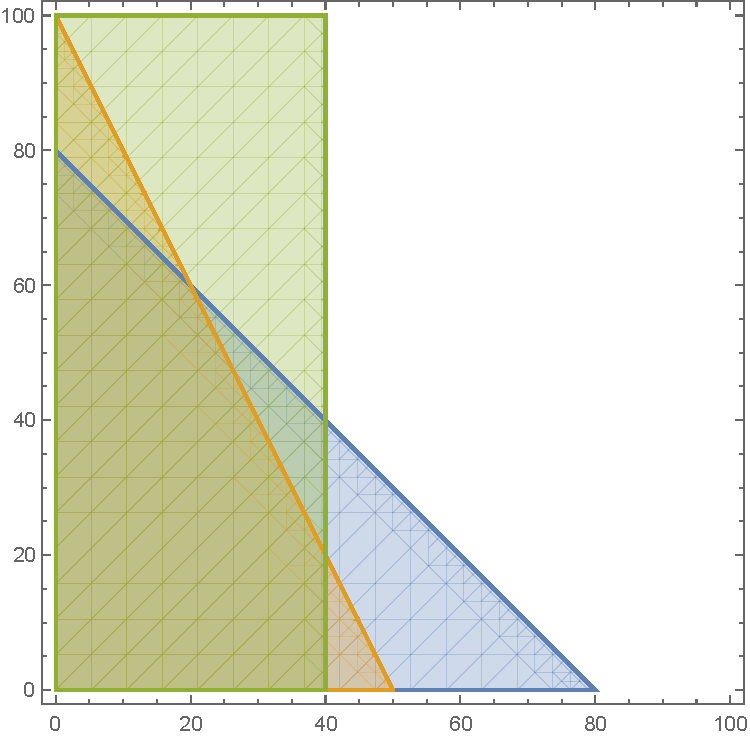
\includegraphics[width=2in]{ResolucionGrafica1}
	\caption[Gráfica de las restricciones de nuestro problema]{Gráfica de las restricciones de nuestro problema}
\end{figure}
Y nos quedamos con la intersección de todas las gráficas:
\begin{figure}[h]
	\centering
	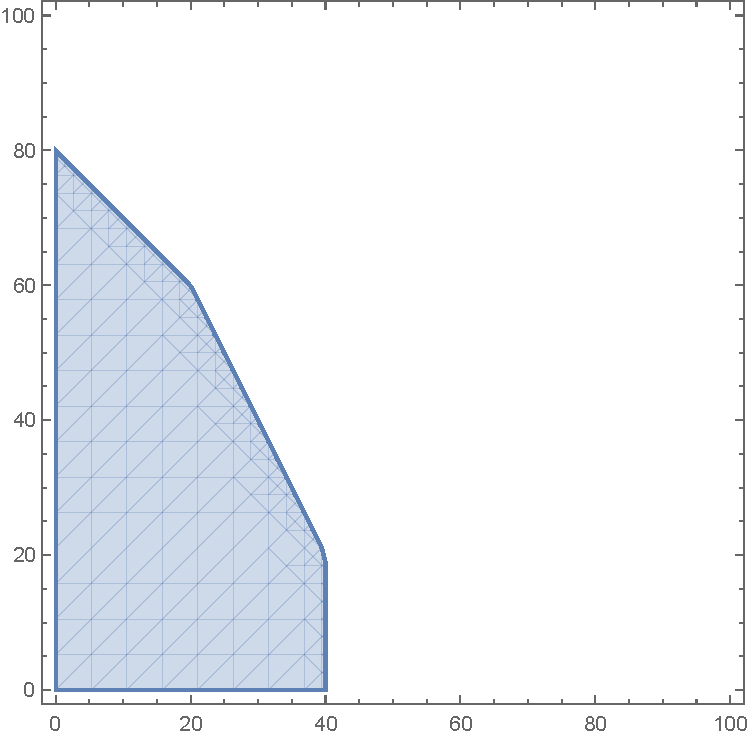
\includegraphics[width=2in]{ResolucionGrafica2}
	\caption[Gráfica de las restricciones de nuestro problema]{Gráfica de las restricciones de nuestro problema}
\end{figure}
Para mejorar nuestra función objetivo debemos movernos de forma perpendicular a la gráfica de la función $3s+2t$, esto es, que debemos movernos en la dirección del vector gradiente de $3s+2t$, esta dirección es $(3, 2)$, por tanto:
\begin{figure}[!ht]
	\centering
	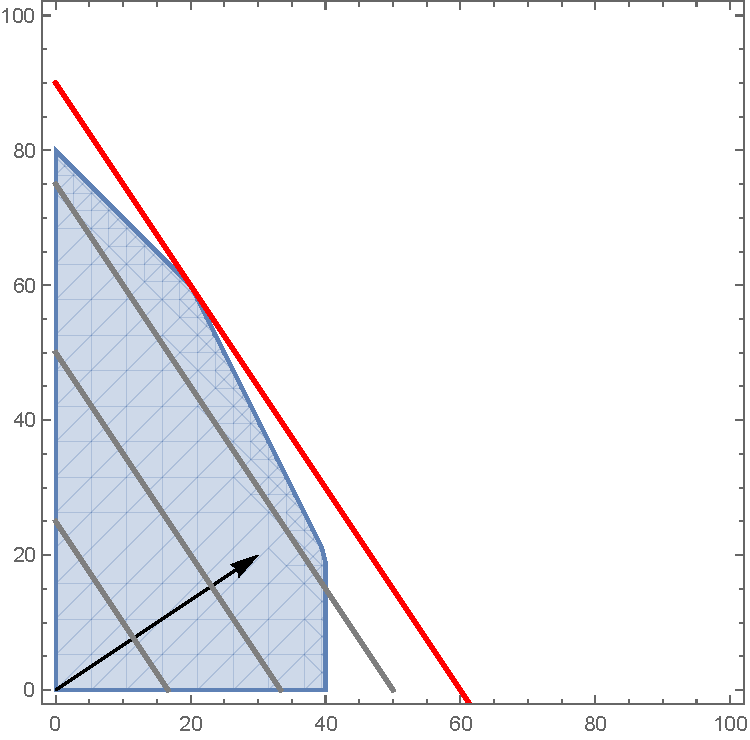
\includegraphics[width=2in]{ResolucionGrafica3}
	\caption[Gráfica de las restricciones de nuestro problema]{Gráfica de las restricciones de nuestro problema}
\end{figure}
\begin{definition}[Restricción activa]
	Se dice que una restricción es activa para un punto $x_0$ si dicha restricción se verifica en forma de igualdad para este punto.
\end{definition}
\section{Clasificación de PPL según sus soluciones}
Dado un PPL, [P], si $R = \emptyset$, \textbf{el problema es infactible}, es decir, \textbf{no tiene solución.} [\ref{fig:Infactible}] \\
Por otro lado, si $R \neq  \emptyset$, podemos asegurar lo siguiente: \\
\textbf{Existen solución: } \\
- Únicas [\ref{fig:Unica}] \\
- Múltiples, es decir, infinitas soluciones que determina el mismo valor de $f$, basta ver el gráfico [\ref{fig:Multiple}] y tomar una función objetivo con un vector gradiente paralelo.\\
\textbf{No acotado: } \\
Existen soluciones factibles que hacen mejorar a la función objetivo todo lo que queramos, basta tomar el vector director de la función paralelo al lado inferior y superior del paralelogramo. \ref{fig:noacotada}
\begin{figure}[ht]
	\centering
	\begin{subfigure}[b]{0.25\textwidth}
		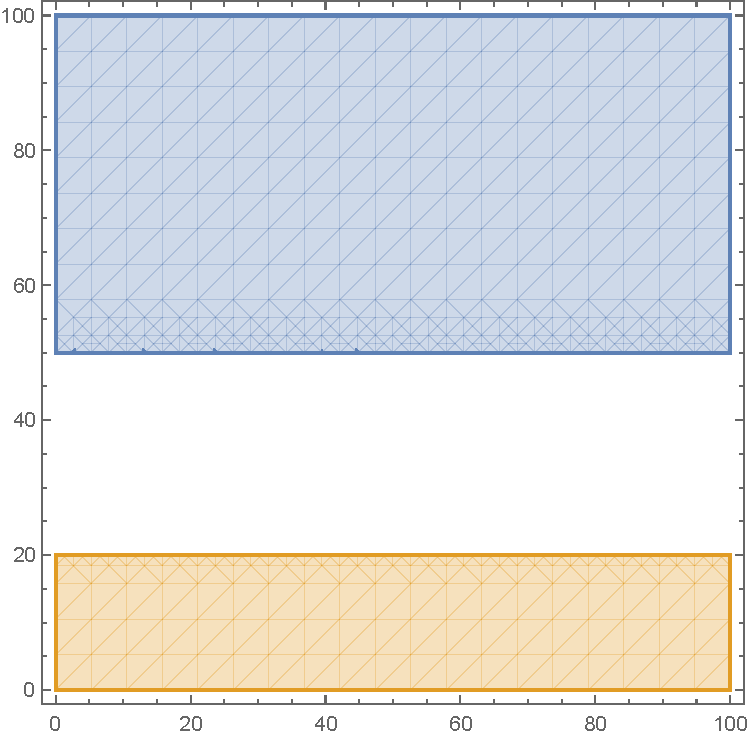
\includegraphics[width=\textwidth]{Infactible}
		\caption{Problema infactible}
		\label{fig:Infactible}
	\end{subfigure}
	\begin{subfigure}[b]{0.25\textwidth}
		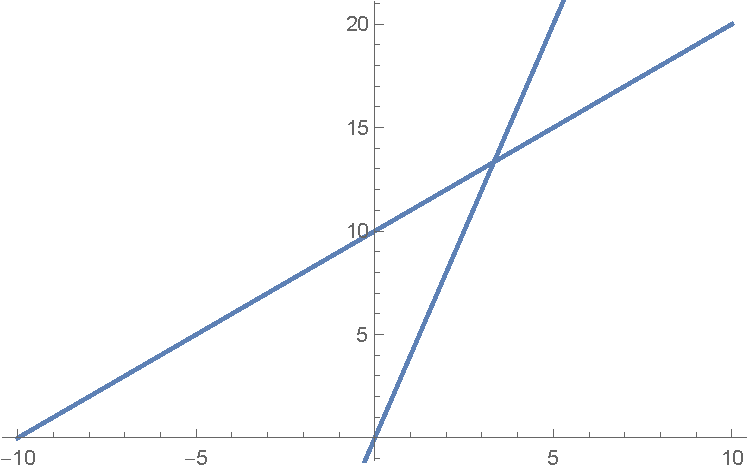
\includegraphics[width=\textwidth]{SolucionUnica}
		\caption{Solución única}
		\label{fig:Unica}
	\end{subfigure}
	\begin{subfigure}[b]{0.25\textwidth}
		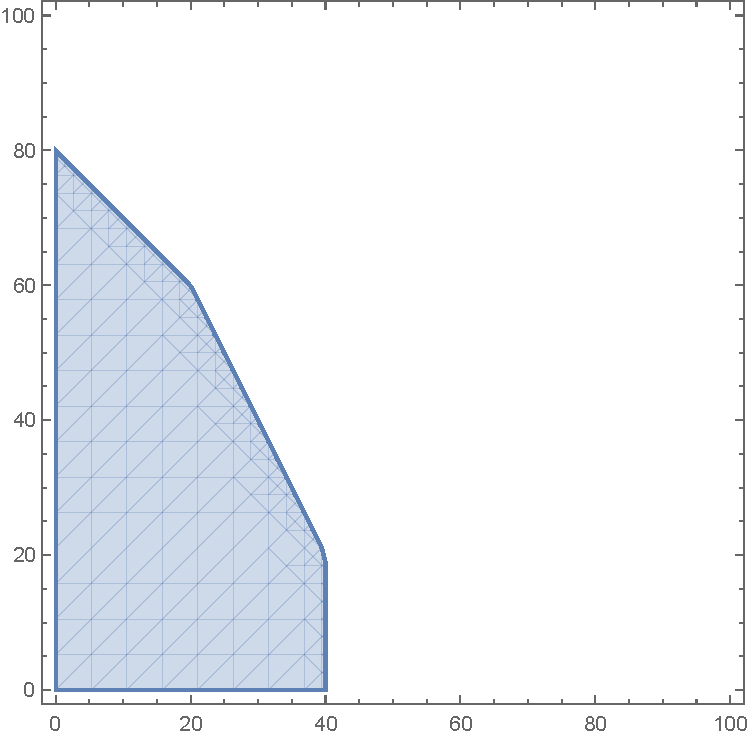
\includegraphics[width=\textwidth]{ResolucionGrafica2}
		\caption{Solución múltiple}
		\label{fig:Multiple}
	\end{subfigure}
	\begin{subfigure}[b]{0.25\textwidth}
		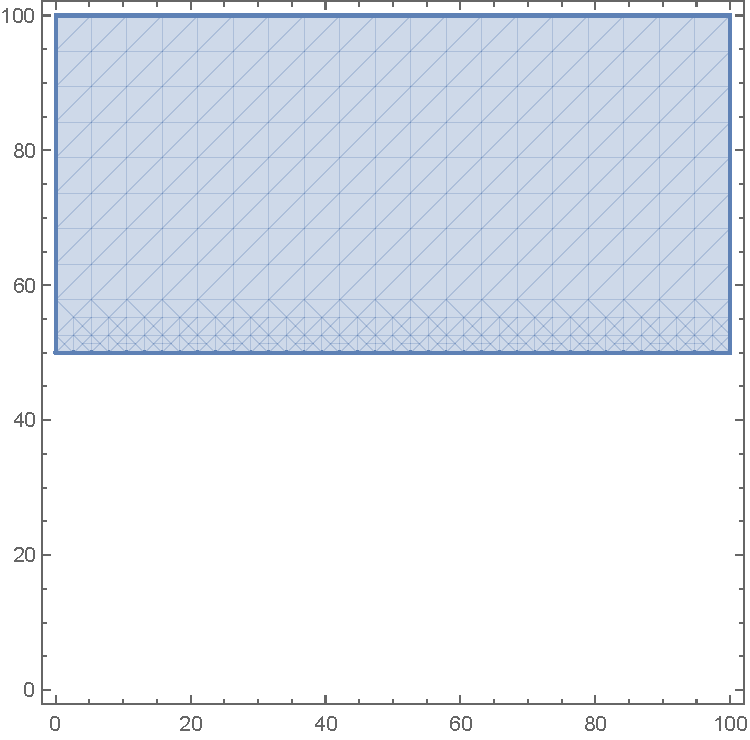
\includegraphics[width=\textwidth]{SolucionNoAcotada}
		\caption{Solución no acotada}
		\label{fig:noacotada}
	\end{subfigure}
	\caption{Clasificación de PPL según sus soluciones}
\end{figure}

\section{Formas geométricas de un PPL}
\begin{definition}[Conjunto convexo]
	Se dice que $S \subset \mathbb{R}^n$ es un conjunto convexo si para todo $x, y \in S$ y $x \neq y$ se verifica $\lambda x + (1-\lambda)y \in S$ para todo $\lambda \in (0, 1)$
\end{definition}
\begin{figure}[h]
	\centering
	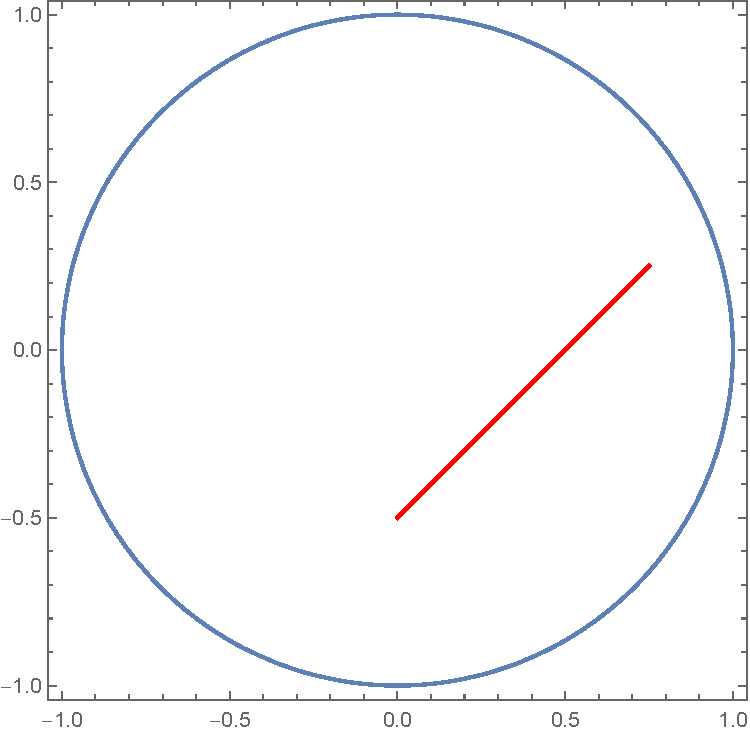
\includegraphics[width=2in]{Convexo}
	\caption[Ejemplo de conjunto convexo]{Ejemplo de conjunto convexo, donde en rojo se indica un camino convexo}
\end{figure}

\begin{proposition}
	La intersección finita de conjuntos convexo es convexo.
\end{proposition}

\begin{proof}
	Sean $\{S_i\}_{i \in I}$ una familia de conjuntos convexos con $|I|<\infty$. \\
	Veamos que la intersección de esta familia de conjuntos sigue siendo convexa. \\
	Sean $x, y \in S=\cap S_i$ con $x \neq y$ entonces $x, y \in S_j$ para algún $j\in I$. \\
	$S_j$ es conexo, por tanto, $\lambda x+(1-\lambda)y \in S_j$, por tanto, $\lambda x+(1-\lambda)y \in S$
\end{proof}

\begin{definition}[Hiperplano en $\mathbb{R}^n$]
	Se llama hiperplano de $\mathbb{R}^n$ el conjunto $\mathcal{H}=\{x \in \mathbb{R}^n : a^t x = b \}$ 
\end{definition}

\begin{definition}[Semiespacio cerrado positivo]
	Se llama semiespacio cerrado positivo el conjunto $\mathcal{H}^+=\{x \in \mathbb{R}^n : a^t x \geq b \}$
\end{definition}
\begin{definition}[Semiespacio cerrado negativo]
	Se llama semiespacio cerrado negativo el conjunto $\mathcal{H}^-=\{x \in \mathbb{R}^n : a^t x \leq b \}$
\end{definition}

\begin{definition}[Polítopo]
	Se llama polítopo de $\mathbb{R}^n$ a la intersección finita de hiperplanos y semiespacios cerrados.
\end{definition}
\textbf{Observación: } Dado un PPL la región factible de $[P]$ es polítopo.

\begin{definition}[Poliedro]
	Cuando el polítopo es acotado se denomina poliedro.
\end{definition}

\begin{proposition}
	Todo polítopo es convexo.
\end{proposition}

\begin{proof}
	Sea $a \in \mathbb{R}^n$, $a \neq 0$ y $b \in \mathbb{R}$. \\
	Por el anterior Lema, seria equivalente a ver si los semiespacios y los hiperplanos son convexos; si vemos esto, ya lo habríamos demostrado. \\
	\textbf{$\mathcal{H}^+$ es convexo: } \\
	Sean $x, y  \in \mathcal{H}^+$, $x \neq y$ tenemos que ver que $\lambda x + (1-\lambda)y \in \mathcal{R}^+$. \\
	Por un lado, si $x \in \mathcal{R}^+$, entonces $a^t x \geq b$. \\
	Por otro lado, si $y \in \mathcal{R}^+$, tenemos que $a^t y \geq b$. \\
	De estas dos observaciones, $a^t(\lambda x + (1-\lambda) y )=\lambda a^t x + (1-\lambda)a^t y \geq \lambda b + (1-\lambda ) b =b$. \\
	Por tanto, $\mathcal{H}^+$ es convexo, para ver si los demás son convexo se realiza de una forma similar a la seguida en esta.
\end{proof}

\begin{definition}[Punto extremo]
	Sea $S \subset \mathbb{R}^n$ un conjunto de $\mathbb{R}^n$, sea $e \in S$, se dice que $e$ es un \textbf{punto extremo} de $S$ si no existen $x , y \in S$, con $x \neq y$ tal que $e= \lambda x + (1-\lambda) y$ para algún $\lambda \in (0, 1)$
\end{definition}

\begin{definition}[Dirección de ilimitación]
	Dado un PPL [P] con $R \neq \emptyset $ la región factible de [P]. \\
	Se dice que $d \in \mathbb{R}^n$ es dirección de ilimitación de $R$ si para cualquier $x_0 \in R$, y cualquier $\lambda \geq 0$ se tiene que $x_0 + \lambda d \in R$.
\end{definition}

\begin{definition}[Dirección de limitación extrema]
	Dado un PPL [P] y $R$ su región factible se dice que $d \in \mathbb{R}^n$, $d \geq 0$, es dirección de limitación extrema no existe $d_1, d_2 \in \mathbb{R}^n$, $d_1, d_2 \geq 0$ direcciones de ilimitación de $R$ tales que $d= \lambda_1 d_1+\lambda_2 d_2$ con $\lambda_1, \lambda_2 \geq 0$. 
\end{definition}
	
\begin{proposition}
	Dado un PPL [P] y $R$ (no acotado) su región factible se tiene que: \\
	$d \in \mathbb{R}^n, d \geq 0$ es dirección de ilimitación si y sólo sí $Ad=0$ 
\end{proposition}

\begin{proof}
	Supongamos que $d$ es dirección de ilimitación de $R$. \\
	
	$\Rightarrow$ \\
	
	Para todo $x_0 \in R$ tenemos que $(x_0+\lambda d) \in R$ para todo $\lambda \geq 0$, por tanto:
	\begin{eqnarray}
		A(x_0+\lambda d) = b \\
		Ax_0+\lambda A d = b
	\end{eqnarray}
	Sabemos que $x_0 \in R$, entonces $Ax_0=b$, de aquí:
	\begin{eqnarray}
	b+\lambda A d = b \\
	\lambda A d = 0
	\end{eqnarray}
	Como la igualdad anterior es para todo $\lambda \geq 0$, necesariamente $Ad=0$. \\
	$\Leftarrow$ \\
	Supongamos que $Ad=0$, ¿Para todo $x_0 \in R$ se cumple que $x_0 + \lambda d  \in R$ para todo $\lambda \geq 0$? \\
	En efecto, escribamos $A(x_0+\lambda d)$, aplicando la propiedad distributiva tenemos: \\
	$Ax_0+A \lambda d=Ax_0+0=Ax_0=b$. ¿$x_0+\lambda d \geq 0$? Sí, $x_0 \in R$, por tanto $x_0, \lambda, d \geq 0$.  
\end{proof}

\section{Hipótesis de rango completo}
Sea [P] un PPL estándar con matriz de coeficientes $A_{mxn}$, $rango(A)=m$, $m\leq n$ \\
$$[A]_{mxn} \cdot [X]_{nx1}=[b]_{mx1}$$
Si $rango(A)<m$ entonces existen $m-rango(A)$ filas linealmente dependientes.
\subsection*{Caso I}
Si el $rango(A)<rango(A|b)$ entonces, no existe solución, por tanto tenemos un problema \textbf{infactible}
\subsection*{Caso II}
Si el $rango(A)=rango(A|b)<m$ entonces tenemos un sistema compatible indeterminado.
\subsection*{Conclusión}
Para evitar trivialidades, en los problemas de teoría supondremos que $rango(A)=m$
\section{Soluciones básicas}
\begin{definition}[Solución básica]
	Supongamos que [P] es un PPL en formato estándar y $rango(A)=m$
	$$ [B ~ N] _{mxn} \cdot \left[\begin{array}{c}
	x_B \\
	x_N
	\end{array}\right]_{nx1}=[b]_{mx1}
	$$
	Suponemos además que $rango(B)=m=rango(B | b)$ entonces tenemos que:
	$ B \cdot x_b=b$ es un sistema compatible determinado.
	
	\begin{enumerate}
		\item Si $m=n$ entonces el sistema es compatible determinado, por la tanto la solución es única.
		\item Si $m<n$ entonces el sistema es compatible indeterminado, de aquí, existen infinitas soluciones.
	\end{enumerate}
	Tomemos ahora el vector $x=\left[\begin{array}{c}
	x_B \\
	0
	\end{array}\right]$, $x \in \mathbb{R}^n$, es \textbf{solución básica} de $[P]$ y se denomina \textbf{solución básica factible.}
	\end{definition}
Recordemos una propiedad de los menores: \\
\textbf{Recordatorio: } Dada una matriz $A$ con $rango(A)=m$ entonces existe un menor de $A$ de orden $m$ A, es decir, existen $m$ columnas independientes. \\
\textbf{Ejemplo: } \\
Sea $3x_1+2x_2$ la función objetivo y sujeto a:
\begin{equation*}
\left\lbrace
\begin{array}{l}
x_1+4x_2 \geq 17 \\
7x_2 \leq 10
\end{array}
\right.
=
\left\lbrace
\begin{array}{l}
x_1+4x_2 -s_1= 17 \\
7x_2 + s_2 = 10
\end{array}
\right.\Rightarrow
\left(\begin{array}{cc|cc}
	1&4&-1&0\\
	0&7&0&1
\end{array}\right)=
\left(\begin{array}{c}
	x_1 \\
	 x_2 \\
	  s_1 \\
	   s_2
\end{array}\right)
=
\left(\begin{array}{c}
17\\10
\end{array}\right)
\end{equation*}
Tenemos que $rango(A)=rango(A | b)=1<4$ número de incógnitas, por tanto si consideramos: \\
$B=\left(\begin{array}{cc}
1&4\\
0&7
\end{array}\right)$, $\left(\begin{array}{cc}
1&4\\
0&7
\end{array}\right)=\left(\begin{array}{c}
x_1 \\
x_2
\end{array}\right)=\left(\begin{array}{c}
17 \\ 10
\end{array}\right)$, por tanto $x_1=\frac{79}{7}, x_2=\frac{10}{7}$, por tanto $(\frac{79}{7}, \frac{10}{7},0,0)^t$ es solución básica. \\
\begin{definition}[Variables básicas]
	Dado [P] un PPL y $x_0$ una solución básica de [P] a las variables de $x_0$ que están asociadas a las columnnas de $B$ se las denomina \textbf{variables básicas}. En caso contrario, \textbf{son variables no básicas}.
\end{definition}
\begin{definition}[Solución básica degenerada]
	Se denomina solución básica degenerada a la solución básica que tiene algunas de sus variables básicas nulas. Las variables no básicas siempre valen cero.
\end{definition}
\begin{definition}[Soluciones adyacentes]
	Dadas dos soluciones básicas de un problema [P] se dice que son adyacentes si sus correspondientes matrices básicas son iguales excepto en una columna.
\end{definition}

\begin{theorem}[Caracterización solución básica]
	Sea [P] un PPL con región factible $R$ se tiene entonces que $x_0$ es solución básica factible si y sólo si $x_0$ es punto extremo de $R$.
\end{theorem}
\begin{proof}
	$\Rightarrow$ \\
	Sea $x_0$ solución básica factible de [P], entonces $x_0 \in R$. Procedamos por reducción al absurdo: \\
	Supongamos que $x_0$ no es punto extremo de $R$, entonces existen $x, y \in R$, con $x \neq y$ tales que $x_0 = \lambda x + (1-\lambda)y, \lambda \in (0, 1)$ \\
	Como $x_0$ es solución básica: \\
	$x_0=\left(\begin{array}{c}
	x_{01} \\
	x_{02} \\
	... \\
	x_{0p} \\
	0 \\
	... \\
	0
	\end{array}\right)$ con $x_{0i} > 0$ para todo $i=1,...,m$. \\
	Supongamos que	$x_0=\left(\begin{array}{c}
	0 \\
	... \\
	0
	\end{array}\right), x_0 \in R$, por tanto: 
	$$
		\left(\begin{array}{c}
		0 \\
		... \\
		0
		\end{array}\right)=\lambda \left(\begin{array}{c}
		x_1 \\
		x_2 \\
		... \\
		x_n
		\end{array}\right)+(1-\lambda)\left(\begin{array}{c}
		y_1 \\
		y_2 \\
		... \\
		y_n
		\end{array}\right), \lambda \in (0, 1)
	$$
	Observemos que $x_0=\lambda x + (1-\lambda )y$, sólo se daría esta igualdad si $x=y=0$, pues $x, y \in R$, por lo que $x, y \geq 0$, esto contradice nuestras hipótesis \\
	Entonces, si $x_0=\left(\begin{array}{c}
	0 \\
	... \\
	0
	\end{array}\right)$ tendríamos un punto extremo. \\
	
	Sean ahora:
	$$x_0=\left(\begin{array}{c}
	x_{01} \\
	x_{02} \\
	... \\
	x_{0p} \\
	0 \\
	... \\
	0
	\end{array}\right) x=\left(\begin{array}{c}
	x_{1} \\
	x_{2} \\
	... \\
	x_{p} \\
	0 \\
	... \\
	0
	\end{array}\right) y=\left(\begin{array}{c}
	y_{1} \\
	y_{2} \\
	... \\
	y_{p} \\
	0 \\
	... \\
	0
	\end{array}\right)$$
	Volviendo al caso general, $x_0=\lambda x + (1-\lambda)y$: \\
	$\left.\begin{array}{c}
		x \in R \Rightarrow Ax=b \\
		y \in R \Rightarrow Ay=b
	\end{array}\right\}=Ax-Ay=0; A(x-y)=0$. \\
	Aplicando el producto de matrices, llegamos ahora:\\ $(x_1-y_1)(a_1)+(x_2-y_2)(a_2)+...+(x_p-y_p)(a_p)=0$, sabemos que $x_0 \in R$, y sabemos que las columnas asociadas a los $p$ primeros vectores son linealmente independientes, por lo tanto, por la independencia de las columnas $a_1, a_2, ..., a_p$, se tiene necesariamente que $x_i-y_i=0$. \\(Dado que al ser linealmente independiente, los coeficientes que multiplican las columnas deben ser obligatoriamente 0), por tanto, $x=y$, esto contradice nuestras hipótesis \\
	$\Leftarrow$ \\
	Usando la misma notación que antes, sea $x_0$ un punto extremo de $R$.
	\begin{enumerate}
		\item Si las columnas de $A$ asociadas a las componentes $x_{0i}$ con $i=1,...p$ son linealmente independientes, estaría demostrado, pues es solución factible que proviene de columnas linealmente independientes.
		\item En caso contrario, se tiene que $a_1, a_2, ..., a_p$ son linealmente dependientes, existen unos escalares no todos nulos $\lambda_1, ..., \lambda_p$ tales que:
		$$
			\lambda_1 a_1+\lambda_2+a_2+...+\lambda_p a_p=0
		$$
		Sea el vector $\lambda \in \mathbb{R}^n$, donde las $p$ primeras componentes coinciden con la igualdad anterior. \\
		Se define: $\left\{
		\begin{array}{c}
		x_0^+=x_0+\varepsilon \lambda \\
		x_0^-=x_0-\varepsilon \lambda
		\end{array}
		 \right.$ con $\varepsilon \geq 0$. \\
		 Queremos encontrar un $\varepsilon>0$ tal que $\begin{array}{c}
		 x_0^+ \in R \\
		 x_0^- \in R
		 \end{array}$, es decir, $\left\{
		 \begin{array}{c}
		 Ax_0^+=b \\x_0^+ \geq 0 \\ Ax_0^-=b \\ x_0^- \geq 0
		 \end{array}\right.$ \\
		 Observemos lo siguiente:
		 $$
			 Ax_o^+=A(x_0+\varepsilon \lambda)=Ax_0+ \varepsilon A \lambda = b
		 $$
		 Por el mismo razonamiento, podemos ver que $Ax_0^-=b$.  \\
		 Veamos que $x_0^+, x_0^- \geq 0$. Lo veremos para $x_0^+$.
		$$
				 x_0^+=x_0+\varepsilon \lambda=\left(\begin{array}{c}
				 x_{01} \\
				 x_{02} \\
				 ... \\
				 x_{0p} \\
				 0 \\
				 ... \\
				 0
				 \end{array}\right)+\varepsilon\left(\begin{array}{c}
				 y_{01} \\
				 y_{02} \\
				 ... \\
				 y_{0p} \\
				 0 \\
				 ... \\
				 0
				 \end{array}\right)
		$$
		 Si \textit{existen} $\lambda_i < 0$ observamos que:
		$$
			 x_{0i}+\varepsilon\lambda_i\Rightarrow\varepsilon=-\frac{x_{0i}}{\lambda_i}
		$$
		 Si tomamos el mínimo de los epsilon, esto es $\varepsilon_1=\min\{-\frac{x_{0i}}{\lambda_i} : \lambda_i < 0\} \Rightarrow x_0^+=x_0+\varepsilon \lambda \in R$, por tanto, para $\varepsilon_1$, se tiene que $x_0^+ \in R$. \\
		 Podemos razonar igual para $x_0^-$ para concluir que $x_0^- \in R$.\\
		 Finalmente, si tomamos $\varepsilon^*=\min\{\varepsilon_1, \varepsilon_2\}$, tenemos que $x_0^+, x_0^- \in R$, pero tenemos que $x_0=\frac{1}{2}x_0^++\frac{1}{2}x_0^-$, es por lo tanto una combinación convexa con $x_0^+ \neq x_0^-$. Por tanto, hemos llegado una contradicción pues $x_0$ es un punto extremo.
	\end{enumerate}
\end{proof}
\begin{theorem}[Teorema fundamental de la programación lineal]
	Sea [P] un PPL en formato estándar.
	\begin{center}
		máx/mín $f(x_1, ..., x_n)=c_1x_1+...+c_nx_n$
	\end{center}
	$$
		s.a \left\{ \begin{array}{c}
		Ax=b \\
		x\geq0
		\end{array}\right.
		\begin{array}{c}
			A\in \mathcal{M}_{mxn}\\
			rango(A)=m\\
			b\geq 0
		\end{array}
	$$
	\begin{enumerate}
		\item Si $x_0$ es solución factible de [P] entonces existe $x_0^*$ solución básica de [P].
		\item Si $x_0$ es solución factible óptima de [P] entonces existe $x_0^*$ solución básica factible óptima de [P]
	\end{enumerate}
\end{theorem}

\begin{proof}
	Para probar este resultado, observemos: 
\begin{enumerate}
	\item Sea $x_0$ solución factible de [P], entonces $x_0$ se puede expresar como \\
	$$x_0=\left(\begin{array}{c}
	x_{01} \\
	x_{02} \\
	... \\
	x_{0p} \\
	0 \\
	... \\
	0
	\end{array}\right) 
	\begin{array}{c}
	x_{0i}>0\\
	1 \leq i \leq p \leq n
	\end{array}
	$$. \\
	Si las columnas de $A$ $a_1, a_2, ..., a_p$ asociadas a las componentes de $x_0$ mayores que cero son linealmente independientes, entonces $x_0$ sería solución factible básica. 	\framebox[1.1\width]{Fin}  \\
	Si por el contrario, $a_1, ..., a_p$ son linealmente dependientes, entonces existen $\lambda_1, \lambda_2, ..., \lambda_p$ escalares no todos nulos tales que:
	$$
		\lambda_1 a_1+\lambda_2 a_2+ ... + \lambda_p a_p=0
	$$
	Sea $\lambda \in \mathbb{R}^n$ el vector formado por $\lambda_i$ con $i=1,...,p$ donde las $n-p$ columnas valen $0$, $x_0^+=x_0+\varepsilon\lambda$, $\varepsilon \geq 0$. \\
	¿$x_0^+ \in R$? \\
	Vamos a repetir el procedimiento que seguimos en la demostración del teorema anterior: \\
	$Ax_0^+=A(x_0+\varepsilon \lambda )=Ax_0+\varepsilon A \lambda=b$ pues $\varepsilon A \lambda=0$ y $Ax_0=b$. \\
	¿$x_0^+ \geq 0$? \\
	Si existen $\lambda_i < 0$, tomamos $\varepsilon_1= \min\{-\frac{x_{0i}}{\lambda_i} : \lambda_i < 0\}$. \\
	Al tomar este $\varepsilon_1$, habría al menos una componente que se anule. \\
	Entonces, $x_0^+=x_0+\varepsilon_1 \lambda$ tiene como mucho $p-1$ componentes mayores que cero, y el resto nulas. Si las componentes columnas de $A$ asociadas a las componentes mayores que son linealmente independientes => fin. \\
	En caso contrario, reiteramos el razonamiento hasta llegar a un conjunto de columnas de $A$ linealmente independientes. \\
	Si todos los $\lambda_i \geq 0$ \\
	$$
		x_0^-=x_0-\varepsilon \lambda_i, \varepsilon \geq 0
	$$
	$$
		Ax_0^-=Ax_0-\varepsilon A \lambda = b
	$$
	Sea $\varepsilon_2=\min\{ \frac{x_{0i}}{\lambda_i} : \lambda_i \geq 0 \}$ tal que $x_0^-=x_0- \varepsilon_2 \lambda$. \\
	Este $x_0^-$ tiene al menos una componente al menos mayor que cero. Reiterando el razonamiento => fin.
	\item La demostración es igual a la anterior hasta donde tomamos $\lambda \in \mathbb{R}^n$, por la demostración anterior, $x_\varepsilon^+, x_\varepsilon^- \in R$ para cierto $\varepsilon \geq 0$. \\
	Sea $z_0=c^t x_0$ el valor de la función objetivo para $x_0$. \\
	Supongamos que [P] es un problema de maximizar.
	$$
		c^t x_\varepsilon^+=c^t(x_0+\varepsilon \lambda)=c^tx_\varepsilon+\varepsilon c^t \lambda=z_0+\varepsilon c^t \lambda
	$$
	$$
		c^t x_\varepsilon^-=c^t(x_0-\varepsilon  \lambda)=c^t x_0-\varepsilon c^t \lambda = z_0- \varepsilon c^t\lambda
	$$
	\framebox[1.1\width]{Caso 1} \par 
	Supongamos que $c^t \lambda >0$ entonces $c^t x_0=z_0< c^t x_\varepsilon^+$, pero esto es una contradicción pues es un problema de maximizar, y como $x_0$ es solución óptima, no puede haber una solución mayor. \\
	\framebox[1.1\width]{Caso 2} \par 
	Supongamos que $c^t \lambda < 0$ entonces $c^tx_0=z_0<c^tx_\varepsilon^-$, que también es una contradicción por el mismo motivo que antes. \\
	\\
	Por lo tanto, $c^t \lambda = 0$, entonces $c^t x_0=c^t x_\varepsilon^+=c^t x_\varepsilon^-=z_0$, por lo que $x_\varepsilon^+$ y $x_\varepsilon^-$ son soluciones factibles óptimas. \\
	Ahora reiteramos el proceso de la primera parte de la demostración y obtendremos $x_\varepsilon^+, x_\varepsilon^-$ soluciones factibles óptimas básicas.
\end{enumerate}
\end{proof}

\begin{corollary}
	Dado un PPL con región factible $R$ se tiene que si $R \neq \emptyset$ entonces siempre existen puntos extremos de $R$.
\end{corollary}
\begin{corollary}
En las mismas condiciones del corolario anterior, si existe solución óptima de [P] entonces existe un punto extremo de $R$ que es solución óptima de [P]
\end{corollary}
\begin{corollary}
	En las mismas condiciones del corolario anterior, el conjunto de puntos extremos de R es finito y a lo sumo tiene $\left(\begin{array}{c}
	n \\ m
	\end{array}\right)$ puntos
\end{corollary}

\section{Método Simplex}
El método Simplex nos calcula soluciones óptimas de un problema, para ello:
\begin{enumerate}
	\item Como cambiar de solución básica adyacente en soluciones básicas adyacentes.
	\item Como conseguir que la solución básica a la que he cambiado sea factible. ($x \geq 0$)
	\item Que variable (columna) debe entrar para mejorar la función objetivo.
\end{enumerate}
\subsection{Pivotar, "saltar" de solución básica factible en solución básica factible}
Sea $[P]$ un PPL en formato estándar:
$$ mín(max) c^t x$$
$$
s.a \left\{\begin{array}{c}
Ax=b \\
x \geq 0
\end{array}\right.
$$
$$ A \in \mathcal{M}_{mxn}, b\geq 0, rango(A)=m$$
Podemos suponer sin perdida de generaldiad que la matriz $A$ se puede escribir como $$[A][x]=[B_{mxn} ~ N_{mx(n-m)}]\left[\begin{array}{c}
x_B \\
x_N
\end{array}\right]=[b]$$
La matriz $B$ es invertible, por tanto podemos multiplicar por $B^{-1}$ y tenemos:
$$[Id_{mxn} ~ N_{mx(n-m)}]\left[\begin{array}{c}
x_B \\
x_N
\end{array}\right]=[B^{-1}][b]$$
\subsubsection{Ejemplo}
$$ máx/min ~c^t x$$
$$s.a \left\{ \begin{array}{c}
x_1+5x_4=57 \\
x_1-4 x_4=12 \\
x_1+x_4 = 5
\end{array}\right.$$
\textbf{Tabla simplex}
$$
\begin{array}{c|cccc|c}
 & x_1 & x_2 & x_3 & x_4 &  \\ \hline
x_1 & 1 & 0 & 0 & 5 & 57 \\
x_2 & 0 & 1 & 0 & -4 & 12 \\
x_3 & 0 & 0 & 1 & 1 & 5 \\ \hline
& & & & &
\end{array}
$$
Supongamos que $x_4$ mejora a la solución actual. Cambiamos por ejemplo, $x_4$ por $x_3$
$$
\begin{array}{c|cccc|c}
& x_1 & x_2 & x_3 & x_4 &  \\ \hline
x_1 & 1 & 0 & 0 & 5 & 57 \\
x_2 & 0 & 1 & 0 & -4 & 12 \\
x_3 & 0 & 0 & 1 & 1 & 5 \\ \hline
& & & & \uparrow &
\end{array}
$$
Hacemos operaciones Gaussianas para poner la columna $x_4$ como básica:
$$
\begin{array}{c|cccc|c}
& x_1 & x_2 & x_3 & x_4 &  \\ \hline
x_1 & 1 & 0 & -5 & 0 & 32 \\
x_2 & 0 & 1 & 4 & 0 & 32 \\
x_4 & 0 & 0 & 1 & 1 & 5 \\ \hline
& & & &  &
\end{array}
$$
Ahora volvemos a la solución básica inicial
$$
\begin{array}{c|cccc|c}
& x_1 & x_2 & x_3 & x_4 &  \\ \hline
x_1 & 1 & 0 & 0 & 5 & 57 \\
x_2 & 0 & 1 & 0 & -4 & 12 \\
x_3 & 0 & 0 & 1 & 1 & 5 \\ \hline
& & & & &
\end{array}
$$
Ahora queremos que entre en la base la variable $x_4$ y que salga la variable $x_2$
$$
\begin{array}{c|cccc|c}
& x_1 & x_2 & x_3 & x_4 &  \\ \hline
x_1 & 1 & \frac{5}{4} & 0 & 0 & 72 \\
x_4 & 0 & -\frac{1}{4} & 0 & 1 & -3 \\
x_3 & 0 & \frac{1}{4} & 1 & 0 & 8 \\ \hline
& & & & &
\end{array}
$$

\subsection{Dada una variable no básica que mejore la solución actual, ¿Qué variable no básica debe salir?}
Sea $[P]$ un PPL en formato estándar:
$$ min ~(max) c^tx$$
$$s.a \left\{ \begin{array}{c}
Ax=b \\x \geq 0
\end{array} \right. $$
La matriz
$$ [A][x]=[b]$$
Podemos reescribirla de forma que
$$[B ~ N]
\left[\begin{array}{c}
x_B \\
x_N
\end{array}
\right]=[b]
$$
Podemos suponer sin pérdida de generalidad que la $$B=I_{mxn}=\left(\begin{array}{cccc}
1 & ... & ... & ... \\
0 & 1 & ... & ... \\
... & ... & ... & ... \\
... & ... &  0  & 1
\end{array}\right)
$$
Podemos escribir en formato tabla en formato simplex:

$$\left[
\begin{array}{cccc}
1 & ... & ... & ... \\
0 & 1 & ... & ... \\
... & ... & ... & ... \\
... & ... &  0  & 1
\end{array} \left| 
\begin{array}{ccccc}
a_{1 ~ m+1} & ... & a_{1q} & ... & a_{1n} \\
a_{2 ~ m+1} & ... & a_{2q} & ... & a_{2n} \\
... & ... & ... & ... & ... \\
a_{m ~ m+1} & ... & a_{mq} & ... & a_{mn}
\end{array}
\right.
\right]=\left[\begin{array}{c}
x_B \\
x_N
\end{array}
\right]=[b]
$$
$$
\begin{array}{c}
 \\ \hline
x_1 \\
... \\
... \\
x_m \\ \hline
~
\end{array}
\left|
\begin{array}{cccc}
x_1 & x_2 & ... & x_m \\ \hline
1 & ... & ... & ... \\
0 & 1 & ... & ... \\
... & ... & ... & ... \\
... & ... &  0  & 1\\ \hline
& & & 
\end{array}
\begin{array}{ccccc}
x_{m+1} & ... & x_q & ... & x_n \\ \hline
a_{1 ~ m+1} & ... & a_{1q} & ... & a_{1n} \\
a_{2 ~ m+1} & ... & a_{2q} & ... & a_{2n} \\
... & ... & ... & ... & ... \\
a_{m ~ m+1} & ... & a_{mq} & ... & a_{mn} \\ \hline
& & & &
\end{array}
\right|
\begin{array}{c}
b \\ \hline
b_1 \\
... \\
... \\
b_m \\ \hline
~
\end{array}
$$
Supongamos que $x_q$ mejora la solución actual, entonces $x_q$ quiere entrar en la base. \\ ¿Qué variable básica $x_1, ..., x_m$ debe salir?
$$b_1(a_1)+b_2(a_2)+...+b_m(a_m)=b $$
$$b_{1~q}(a_1)+b_{2~q}(a_2)+...+b_{m~q}(a_m)=b $$
$$
b_1a_1+b_2a_2+...+b_na_m=b ~ (1)
$$
$$
a_{1~q}a_1+a_{2~q}a_2+...+a_{n~q}a_m=a_q ~(2)
$$
Sea $\varepsilon\geq0$ y realicemos la siguiente operación:
$$(1)-\varepsilon(2)$$
$$(b_1-\varepsilon a_{1 ~ q})a_1+(b_2-\varepsilon a_{2 ~ q})+...+(b_m-\varepsilon a_{m ~q})a_m=b-\varepsilon a_q$$
$$(b_1-\varepsilon a_{1 ~ q})a_1+(b_2-\varepsilon a_{2 ~ q})+...+(b_m-\varepsilon a_{m ~q})a_m+\varepsilon a_q=b$$
Definamos ahora el vector:
$$
x_\varepsilon=\left(
\begin{array}{c}
b_1-\varepsilon a_{1 ~ q} \\
b_2-\varepsilon a_{2 ~ q} \\ 
... \\
b_m-\varepsilon a_{m ~ q} \\
... \\
\varepsilon \\
... \\
0
\end{array}
\right)
\left(
\begin{array}{c}
1 \\
2 \\
... \\
m \\
... \\
q \\
... \\
0
\end{array}
\right)
$$
\textbf{Caso I: } Si $a_{iq}<0$ para $1\leq i \leq m$, entonces $x_\varepsilon \in R$ para todo $\varepsilon \geq 0$. \\
En este caso, el problema es no acotado, encuentro una solución que hace que la función objetivo mejore todo lo queramos. \\
\textbf{Caso II: } Si existen algunos $a_{iq}>0$, queremos que:
$$b_i-\varepsilon a_{iq}=0$$
Tomando $$\varepsilon=\min\{\frac{b_i}{a_{i1}} : a_{iq} > 0\}$$ \\
Entonces entra en la base la variable $x_q$, sale de la base la variable asociada a la ecuación $b_i-\varepsilon a_{iq}=0$ (En caso de empate, puede salir la que queramos)
\subsubsection{Forma alternativa de la fase II}
Supongamos que $x_q$ entra en la base y que $x_k$ es la variable básica que debe salir.
$$
\begin{array}{c}
\\ \hline
x_1 \\
... \\
... \\
\leftarrow x_k \\
... \\
x_m \\ \hline
~
\end{array}
\left|
\begin{array}{cccccc}
x_1 & x_2 & ... & x_k & ... & x_m \\ \hline
1 & ... & ... &...& ...& ... \\
0 & 1 & ... & ...& ...& ... \\
... & ... & ... & ... & ...& ... \\
... & ... & ... & 1 & ...& ... \\
... & ... & ... & ... & ...& ... \\
... & ...& .... & ... &  0  & 1\\ \hline
& & & 
\end{array}
\begin{array}{ccccc}
x_{m+1} & ... & x_q & ... & x_n \\ \hline
a_{1 ~ m+1} & ... & a_{1q} & ... & a_{1n} \\
a_{2 ~ m+1} & ... & a_{2q} & ... & a_{2n} \\
... & ... & ... & ...& ... \\
... & ... & a_{kq} & ...& ... \\
... & ... & ... & ...& ... \\
a_{m ~ m+1} & ... & a_{mq} & ... & a_{mn} \\ \hline
& & & &
\end{array}
\right|
\begin{array}{c}
b \\ \hline
b_1 \\
... \\
... \\
b_k \\
... \\
b_m \\ \hline
~
\end{array}
$$
Aplicamos operaciones Gaussianas
$$F_k'=\frac{1}{a_{kq}}F_k$$

$$
\begin{array}{c}
\\ \hline
x_1 \\
... \\
... \\
\leftarrow x_k \\
... \\
x_m \\ \hline
~
\end{array}
\left|
\begin{array}{cccccc}
x_1 & x_2 & ... & x_k & ... & x_m \\ \hline
1 & ... & ... &...& ...& ... \\
0 & 1 & ... & ...& ...& ... \\
... & ... & ... & ... & ...& ... \\
... & ... & ... & \frac{1}{a_{kq}}  & ...& ... \\
... & ... & ... & ... & ...& ... \\
... & ...& .... & ... &  0  & 1\\ \hline
& & & 
\end{array}
\begin{array}{ccccc}
x_{m+1} & ... & x_q & ... & x_n \\ \hline
a_{1 ~ m+1} & ... & a_{1q} & ... & a_{1n} \\
a_{2 ~ m+1} & ... & a_{2q} & ... & a_{2n} \\
... & ... & ... & ...& ... \\
... & ... & \frac{a_{kq}}{a_{kq}} & ...& ... \\
... & ... & ... & ...& ... \\
a_{m ~ m+1} & ... & a_{mq} & ... & a_{mn} \\ \hline
& & & &
\end{array}
\right|
\begin{array}{c}
b \\ \hline
b_1 \\
... \\
... \\
\frac{b_k}{a_{kq}} \\
... \\
b_m \\ \hline
~
\end{array}
$$
Hacemos ahora la siguiente operación:
$$F_j=F_j - a_{jq}F_k ~ \forall j\neq q$$

$$
\begin{array}{c}
\\ \hline
x_1 \\
... \\
... \\
\leftarrow x_k \\
... \\
x_m \\ \hline
~
\end{array}
\left|
\begin{array}{cccccc}
x_1 & x_2 & ... & x_k & ... & x_m \\ \hline
1 & ... & ... &...& ...& ... \\
0 & 1 & ... & ...& ...& ... \\
... & ... & ... & ... & ...& ... \\
... & ... & ... & ...  & ...& ... \\
... & ... & ... & ... & ...& ... \\
... & ...& .... & ... &  0  & 1\\ \hline
& & & 
\end{array}
\begin{array}{ccccc}
x_{m+1} & ... & x_q & ... & x_n \\ \hline
a_{1 ~ m+1} & ... & a_{1q} & ... & a_{1n} \\
a_{2 ~ m+1} & ... & a_{2q} & ... & a_{2n} \\
... & ... & ... & ...& ... \\
... & ... & 1 & ...& ... \\
... & ... & ... & ...& ... \\
a_{m ~ m+1} & ... & a_{mq} & ... & a_{mn} \\ \hline
& & & &
\end{array}
\right|
\begin{array}{c}
b \\ \hline
b_1 - a_{1q}\frac{b_k}{a_{kq}}\\
... \\
... \\
\frac{b_k}{a_{kq}} \\
... \\
b_m- a_{mq}\frac{b_k}{a_{kq}} \\ \hline
~
\end{array}
$$
Como $b_i \geq 0$ entonces, $a_{kq}>0$ de modo que 
$$ b_i-a_{iq}\frac{b_k}{a_{kq}} \geq 0 $$
$$ b_i\geq a_{iq}\frac{b_k}{a_{kq}} $$
\begin{enumerate}
	\item Si $a_{iq}$ para todo $i=1,...,m$ para $i \neq k$ entra la nueva solución factible
	\item Si existen algunos $a_{iq}>0$
	$$ b_i-a_{iq}\frac{b_k}{a_{kq}} \geq 0 $$
	$$ b_i\geq a_{iq}\frac{b_k}{a_{kq}} $$
	Dado que $ a_{iq}>0$
	$$ \frac{b_i}{ a_{iq}}\geq\frac{b_k}{a_{kq}} $$
\end{enumerate}
La fila asociada a $\displaystyle\min\{\frac{b_i}{a_{iq}}: a_{iq}>0\}$ indica la variable que debe salir.

\subsection{¿Qué variable no básica mejora a la solución actual?}
Partimos del siguiente sistema:
$$
\begin{array}{c}
\\ \hline
x_1 \\
... \\
... \\
x_k \\
... \\
x_m \\ \hline
~
\end{array}
\left|
\begin{array}{cccccc}
x_1 & x_2 & ... & x_k & ... & x_m \\ \hline
1 & ... & ... &...& ...& ... \\
0 & 1 & ... & ...& ...& ... \\
... & ... & ... & ... & ...& ... \\
... & ... & ... & 1 & ...& ... \\
... & ... & ... & ... & ...& ... \\
... & ...& .... & ... &  0  & 1\\ \hline
& & & 
\end{array}
\begin{array}{ccccc}
x_{m+1} & ... & x_q & ... & x_n \\ \hline
a_{1 ~ m+1} & ... & a_{1q} & ... & a_{1n} \\
a_{2 ~ m+1} & ... & a_{2q} & ... & a_{2n} \\
... & ... & ... & ...& ... \\
... & ... & a_{kq} & ...& ... \\
... & ... & ... & ...& ... \\
a_{m ~ m+1} & ... & a_{mq} & ... & a_{mn} \\ \hline
& & & &
\end{array}
\right|
\begin{array}{c}
b \\ \hline
b_1 \\
... \\
... \\
b_k \\
... \\
b_m \\ \hline
~
\end{array}
$$
La solución básica asociada a la tabla anterior viene dada por:
$$
x_0=\left(
\begin{array}{c}
b_1 \\
b_2 \\
... \\
b_m \\
0 \\
... \\
0
\end{array}
\right)
$$
Sea $f(x_1, x_2, ..., x_n)=c_1 x_1+...+c_n x_n$ para $c_i \in \mathbb{R}$ para todo $i=1, ..., n$ \\
\textbf{¿Qué valor alcanza $x_0$ en la función objetivo?}
$$f(x_1, x_2, ..., x_n)=c_1 x_1+...+c_m x_m+c_{m+1} \cdot 0+...+c_n \cdot 0=z_0$$
Vamos a despejar los $x_i$ para $i=1, ..., m$ en términos del resto de variables.
$$
\left\{
\begin{array}{c}
\displaystyle x_1=b_1-\sum_{j=m+1}^{n}a_{1j}x_j \\
\displaystyle x_2=b_2-\sum_{j=m+1}^{n}a_{2j}x_j \\
... \\
\displaystyle x_m=b_m-\sum_{j=m+1}^{n}a_{mj}x_j \\
\end{array}
\right.
$$ 
\textbf{¿Qué valor alcanza la función objetivo en la solución general $x$?}
$$f(x_1, x_2, ..., x_n)=c_1 (b_1-\sum_{j=m+1}^{n}a_{1j}x_j)+c_2 (b_2-\sum_{j=m+1}^{n}a_{2j}x_j)+...+c_m (b_m-\sum_{j=m+1}^{n}a_{mj}x_j)+x_{m+1}c_{m+1}+...+c_n x_n$$
Aplicando la propiedad distributiva ahora:
$$f(x_1, x_2, ..., x_n)=c_1 (b_1-\sum_{j=m+1}^{n}a_{1j}x_j)+c_2 (b_2-\sum_{j=m+1}^{n}a_{2j}x_j)+...+c_m (b_m-\sum_{j=m+1}^{n}a_{mj}x_j)+x_{m+1}c_{m+1}+...+c_n x_n=$$
$$=c_1b_1+c_2+...+c_mb_m-c_1\sum_{j=m+1}^{n}a_{1j}x_j-c_2\sum_{j=m+1}^{n}a_{2j}x_j-...-c_m\sum_{j=m+1}^{n}a_{mj}x_j+x_{m+1}c_{m+1}+...+c_n x_n=$$
$$=z_0+\left[c_{m+1}-\sum_{i=1}^{m}c_i a_{i~m+1}\right]x_{m+1}+\left[c_{m+2}-\sum_{i=1}^{m}c_ia_{i~m+2}\right]x_{m+2}+...+\left[c_n-\sum_{i=1}^{m}c_ia_{in}\right]x_n=$$
$$=z_0-\left[\sum_{i=1}^{m}c_i a_{i~m+1}-c_{m+1}\right]x_{m+1}-\left[\sum_{i=1}^{m}c_ia_{i~m+2}-c_{m+2}\right]x_{m+2}-...-\left[\sum_{i=1}^{m}c_ia_{in}-c_n\right]x_n=$$
Definimos $r_q=\displaystyle \sum_{i=1}^{m}c_ia_{i~q}-c_{q}$ como costo relativo asociado a la variable $x_i$
\newpage
\begin{theorem}
	Dado un PPL 
	$$min (max) ~ c^t x $$
	$$s.a \left\{ \begin{array}{c}
	Ax=b \\
	x\geq 0
	\end{array}\right.$$
	Si $x_0$ es una solución básica factible de [P] entonces
	\begin{enumerate}
		\item Si todos los costos relativos $r_j$ de las variables básica son positivas o nulas (negativas o nulas) en el caso de maximizar (en el caso de minimizar) entonces $x_0$ es solución óptima de [P].
		\item Si alguno de los costos relativos es negativo (positivo) en el caso de maximizar (minimizar) entonces la solución actual no es óptima y la variable asociada a dicho coste relativo mejorará la solución actual.
		\begin{enumerate}
			\item Si existe $\varepsilon\{\frac{b_i}{a_{ij}} : a_{ij} >0 \}$ entonces la variable que debe de salir es aquella asociada a la fila donde se alcanza el mínimo, $\varepsilon$
			\item Si todos los componentes $a_{ij}<0$ asociados a la variable que \textit{entrar} entrar entonces el problema es no acotado. Podemos encontrar entonces una dirección de ilimitación.
		\end{enumerate}
	\end{enumerate}
	Recordemos, $$r_j=\sum_{i=1}^{m}c_i a_{ij}-c_j$$ 
	Los costos relativos asociados a las variables básicas siempre es $0$.
\end{theorem}

\section{Resolución de un PPL aplicando el Método Simplex}
\subsection{Problema de los soldados y trenes}
$$ max ~ 3x_1+2x_2 $$
$$ s.a \left\{
\begin{array}{c}
2x_1+x_2 \leq 100 \\
x_1+x_2 \leq 80 \\
x_1 \leq 40
\end{array}
\right.
$$
$$ x_1, x_2 \geq 0$$
En primer lugar, escribimos el problema en formato estándar:
$$ max ~ 3x_1+2x_2 $$
$$ s.a \left\{
\begin{array}{c}
2x_1+x_2 + s_1 = 100 \\
x_1+x_2 + s_2 =  80 \\
x_1 + s_3 =  40
\end{array}
\right.
$$
$$ x_1, x_2, s_1, s_2, s_3 \geq 0$$
Escribimos la tabla simplex:
$$
\begin{array}{c|ccccc|c}
& x_1 & x_2 & s_1 & s_2 & s_3 & b \\ \hline
s_1 & 2 & 1 & 1 & 0 & 0 & 100 \\
s_2 & 1 & 1 & 0 & 1 & 0 & 80 \\
s_3 & 1 & 0 & 0 & 0 & 1 & 40 \\ \hline
\end{array}
$$
En este caso, la solución básica actual es: $x_0^t=(0, 0, 100, 80, 40)$. \newpage
Calculamos ahora los costos relativos:
\begin{enumerate}
	\item En cada variable escribimos su coste asociado.
	\item En las variables básica se escribe también su coste relativo.
	\item Multiplicamos los costos escritos en las variables básica con el valor asociado en la matriz en la misma fila y columna, y a continuación, restamos el coste asociado a la variable de la columna.
\end{enumerate}
$$
\begin{array}{c|ccccc|c}
& 3 & 2 & 0 & 0 & 0 & \\
& x_1 & x_2 & s_1 & s_2 & s_3 & b \\ \hline
0 ~ s_1 & 2 & 1 & 1 & 0 & 0 & 100 \\
0 ~s_2 & 1 & 1 & 0 & 1 & 0 & 80 \\
0 ~ s_3 & 1 & 0 & 0 & 0 & 1 & 40 \\ \hline 
& -3 & -2 & 0 & 0 & 0 & 0
\end{array}
$$
Quiere entrar la variable $x_1$ por ser la más negativa, calculamos $100/2$, $80/1$ y $40/1$ dado, que $40/1$ es el mínimo debe salir $s_3$. \\
Debemos convertir la columna asociada a la vaariable $x_1$ en $(0, 0, 1)^t$.
$$F_1'=F_1-2F_3$$
$$F_2'=F_2'-F_3$$
$$
\begin{array}{c|ccccc|c}
& 3 & 2 & 0 & 0 & 0 & \\
& x_1 & x_2 & s_1 & s_2 & s_3 & b \\ \hline
0 ~s_1 & 0 & 1 & 1 & 0 &-2 & 20 \\
0~ s_2 & 0 & 1 & 0 & 1 & -1 & 40 \\
3 ~x_1 & 1 & 0 & 0 & 0 & 1 & 40 \\ \hline 
& 0 & -2 & 0 & 0 & 3 & 120
\end{array}
$$
Quiere entrar la variable $x_2$ por ser la más negativa, calculamos $20/1$, $40/1$ dado, que $20/1$ es el mínimo debe salir $s_1$. \\
Debemos convertir la columna asociada a la variable $x_2$ en $(1, 0, 0)^t$.
$$
\begin{array}{c|ccccc|c}
& 3 & 2 & 0 & 0 & 0 & \\
& x_1 & x_2 & s_1 & s_2 & s_3 & b \\ \hline
2 ~x_1 & 0 & 1 & 1 & 0 &-2 & 20 \\
0~ s_2 & 0 & 0 & -1 & 1 & -1 & 20 \\
3 ~x_1 & 1 & 0 & 0 & 0 & 1 & 40 \\ \hline 
& 0 & 0 & 2 & 0 & -1 & 160
\end{array}
$$
\end{document}
